\documentclass[11pt]{article}

\usepackage[review]{acl}
\usepackage{times}
\usepackage{latexsym}
\usepackage[utf8]{inputenc}
\usepackage[T1]{fontenc}
\usepackage{booktabs}
\usepackage{amsmath}
\usepackage{amssymb}
\usepackage{microtype}
\usepackage{xcolor}
\usepackage{graphicx}
\usepackage{CJKutf8}
\usepackage{enumitem}
\usepackage{float}
\usepackage{natbib}

\title{First-Token Broadcasters: Mechanistic Analysis of Language Identity
and Distributed Robustness in Transformers}

\author{
  Arjun Pillai \\
  \small Irvington High School
  \and
  Christian Hoang \\
  \small Gen4AIE
  \and
  Anjelo Laroza \\
  \small Independent Researcher
}
\begin{document}

\maketitle

\begin{abstract}
How is language identity represented and causally maintained in transformers,
and to what extent do the mechanisms identified in one language set transfer
to other languages and training regimes? We introduce \textbf{Language
Identity Head Ablation (LIHA)}, a causal intervention that zeros each
attention head individually and measures the resulting language switch rate.
Across our multilingual evaluation sets, LIHA identifies heads whose ablation
has disproportionate effects on output language. In GPT-2, a small set of
\emph{first-token broadcaster} heads---led by L6H1 (switch rate 0.32,
3.23$\sigma$ above the population mean)---attend persistently to the first
prompt token across generation steps. The combination of persistent
first-token attention and causal sensitivity suggests that these heads
participate in maintaining output language. Following ablation, we observe
statistically significant redistribution of first-token attention
($p < 10^{-5}$) toward heads in higher layers for the ablations tested;
this pattern is consistent with downstream compensation, although attention
redistribution alone does not establish a feedforward causal cascade. We
also compare Qwen2.5-1.5B-Base and Qwen2.5-1.5B-Instruct, which are matched
in architecture and parameter count but differ in training history. The base
model is nearly flat (max SR$=$0.016, 200/336 heads at SR$=$0.0), whereas the
instruct model concentrates causal influence at layer~0, led by L0H5
(SR$=$0.224, 8.93$\sigma$ above mean). Finally, GPT-2 heads identified from
the European-language experiments show no observed switch effects on the
tested Chinese and Russian prompts, while other early-layer heads do show
effects. Because script, typology, and tokenization vary together in this
comparison, these results do not isolate a specifically script-driven
mechanism.
\end{abstract}

\section{Introduction}

Whether foundation models represent language identity as a single
language-universal signal or as script- and family-specific circuitry
is a question with direct typological stakes: a mechanism identified
on one language family may simply not exist, in any recoverable form,
for a typologically distant one. In GPT-2, a small set of attention heads attend strongly to the first
prompt token across generation steps. For prompts whose first token is
language-informative, these heads show persistent first-token attention. We
call these \emph{first-token broadcaster} heads.

Language confusion has been documented behaviorally across multilingual
models \citep{marchisio-etal-2024-understanding}, while related work has
studied code-switching limitations and language-dependent internal
representations \citep{wendler-etal-2024-llamas}. Prior mechanistic work has also identified
language-specific neurons and shown that manipulating them can influence
generation language \citep{tang-etal-2024-language}. We take a
complementary approach at the attention-head level: for each attention
head, we zero its output during generation and directly measure how often
the output language changes. This causal lens reveals not just which heads
matter, but how language identity is organized across heads and how that
organization changes across training regimes.

Our main findings: \textbf{(1)} partial localization in GPT-2, led by
L6H1 (SR$=$0.32, 3.23$\sigma$ above mean; \S\ref{sec:ablation});
\textbf{(2)} first-token broadcasting, with top heads attending to the
first prompt token at mean weight 0.85--0.94 every step
(\S\ref{sec:attention}); \textbf{(3)} hierarchical compensatory
redistribution ($p<10^{-5}$), recruiting heads \emph{above} the
ablated layer in all three ablated heads tested (\S\ref{sec:multi}); \textbf{(4)} convergent probing
evidence at the same layers (\S\ref{sec:probing}); \textbf{(5)}
instruction tuning reorganizes the circuit toward a sharp layer-0
concentration in Qwen2.5-1.5B-Instruct (14$\times$ higher max SR,
8.93$\sigma$) versus a near-flat base model (\S\ref{sec:qwen});
\textbf{(6)} the European-language broadcaster heads identified in GPT-2 do not
show switch effects on the tested Chinese or Russian prompts, which instead
show effects in other early-layer heads (layers 0--4)
(\S\ref{sec:extended}).

\paragraph{Contributions.} (a) We introduce LIHA as a head-level causal
intervention for measuring changes in output language following attention-head
ablation; (b) we identify GPT-2 heads whose causal influence coincides with
persistent attention to the first prompt token; (c) we characterize
first-token attention redistribution following ablation and test its layerwise
directionality; (d) we compare matched Qwen2.5-1.5B base and instruct variants
and find stronger localization of causal effects in the instruct model; and
(e) we show that European-language broadcaster heads identified in GPT-2 do
not generalize unchanged to the tested Chinese and Russian prompts. The BLOOM
analysis is an exploratory cross-architecture comparison because only every
third layer is sampled.

\section{Related Work}

\citet{elhage2021} established the residual stream framework used
throughout this work; \citet{wang2022interpretability} traced a
26-head circuit for indirect object identification in GPT-2;
\citet{conmy2023towards} introduced automated circuit discovery; and
\citet{meng2022} localized factual associations to MLP modules. On the
multilingual side, \citet{conneau2020} showed multilingual BERT
acquires cross-lingual structure without explicit supervision, and
\citet{marchisio-etal-2024-understanding} document that state-of-the-art
models frequently switch to unintended languages; we approach this
mechanistically via causal ablation rather than behavioral analysis.
\citet{tang-etal-2024-language} identified language-specific neurons via
activation analysis---a language-\emph{selective} signal that need not
coincide with the language-\emph{causal} heads LIHA isolates. On the
typological side, \citet{pires2019multilingual} showed multilingual
BERT's cross-lingual transfer degrades with typological distance
between languages, and \citet{chi2020finding} located universal
grammatical-relation structure within its representations; LIHA
complements this line of work by asking not whether cross-lingual
structure exists, but which specific components causally determine
\emph{which} language identity is broadcast. Linear
probing \citep{alain2016, tenney2019} provides convergent evidence
(\S\ref{sec:probing}), and inference-time steering
\citep{zou2023, li2023} motivates our amplification experiments
(\S\ref{sec:multi}).

\section{Experimental Setup}
\label{sec:setup}

\paragraph{Models and implementation.} GPT-2 small \citep{radford2019}
has 12 layers, 12 heads, and 144 total heads. Qwen2.5-1.5B
\citep{qwen2025} has 28 layers, GQA (2 KV heads, 12 Q heads), and 336
total heads; we compare its base and instruct variants, matched in
architecture and parameter count but differing in training history. For cross-architecture
replication, we additionally evaluate BLOOM-1b7 \citep{bigscience2022bloom},
a model deliberately pretrained on 46 natural languages; it has 24 layers,
16 heads per layer (hidden dim 1024, head dim 64), and 384 total heads.
Each head's output
is isolated by zeroing its post-projection contribution to the residual
stream \citep{elhage2021}, implemented via PyTorch forward hooks on
\texttt{o\_proj}. We use \texttt{langdetect} \citep{shuyo2010} for
language classification and generate 40 tokens per prompt with greedy
decoding.



\paragraph{Dataset.} We construct a multilingual evaluation set drawn from
FLORES-200 \cite{nllbteam2022noLanguageLeftBehind}, spanning five European
languages (English, French, German, Spanish, Italian; 500 sentences each for GPT-2 and 25 sentences per language for Qwen. Chinese
and Russian use 100 sentences each in the extended experiments. The 125 Qwen prompts are a subset
of the 2,500 European-language prompts rather than additional prompts.
Prompts are filtered for quality and verified via 3-way majority vote
(\texttt{langdetect}, \texttt{langid} \citep{lui-baldwin-2012-langid}, fastText \citep{joulin2016fasttext});
all European languages achieved $\geq$99.6\% verified prompts.

\paragraph{Formal definition of LIHA.} Let $\mathcal{M}$ be a
transformer with $L$ layers and $H$ heads per layer. For head
$h_{l,i}$, define the ablated model $\mathcal{M}^{-h_{l,i}}$ as
$\mathcal{M}$ with that head's residual stream contribution set to
zero. The \textbf{switch rate} over prompt set
$\mathcal{X}=\{x_1,\ldots,x_n\}$ is:
\begin{equation}
    S(h_{l,i}) = \frac{1}{n} \sum_{j=1}^{n}
    \mathbf{1}\!\left[\mathcal{L}(\mathcal{M}^{-h_{l,i}}(x_j)) \neq
    \mathcal{L}(\mathcal{M}(x_j))\right]
    \label{eq:switch_rate}
\end{equation}
A head with high $S(h_{l,i})$ has greater causal influence on detected
output-language changes under this intervention. This measure does not imply
that the head uniquely encodes language identity or that it specifically
promotes the target language rather than suppressing alternatives.

\paragraph{Protocols.} We sweep all 144 GPT-2 heads and all 336
Qwen2.5-1.5B heads (both variants); for BLOOM we sweep every third layer
(128 heads). Switch rates report 95\% bootstrap CIs (10,000 samples);
attention redistribution following ablation uses 100,000-sample permutation
tests on first-token attention weight deltas. Zero-ablation is a commonly used
intervention in mechanistic interpretability
\citep{elhage2021, wang2022interpretability}; we discuss mean ablation
as an alternative in \S\ref{sec:limitations}.

\paragraph{Compute and reproducibility.}
All experiments were conducted on a system equipped with an NVIDIA GeForce
RTX~3060 GPU using Python~3.12 and PyTorch. Package dependencies are specified
in the accompanying repository's \texttt{requirements.txt}. Experiments cover
seven languages: English, French, German, Spanish, Italian, Chinese, and
Russian. Generation uses greedy decoding (\texttt{do\_sample=False}), making
generation deterministic for a fixed model and input. Randomized statistical
procedures, including bootstrap and permutation analyses, use random seed~42;
the probing classifier likewise uses \texttt{random\_state=42}. We additionally
set \texttt{DetectorFactory.seed=0} to make \texttt{langdetect} deterministic.
The accompanying repository provides the code, dependency specification, and
experiment scripts required to reproduce the reported results.

\section{Results: Single-Head Ablation and Distributed Robustness (GPT-2)}
\label{sec:ablation}

Figure~\ref{fig:gpt2_ablation} shows the
language switch rate across all 144 GPT-2 heads, sparse with elevated
rates in a cluster spanning layers 0--10. The mean switch rate is 0.163
($\sigma{=}0.049$). L6H1 leads at SR$=$0.32 (99.3rd percentile,
3.23$\sigma$ above mean), the highest-ranked head by both switch rate
and effect size; a second tier (L0H4, L3H1, L9H9) sits at 0.28, with
95\% bootstrap CIs overlapping L6H1's (Table~\ref{tab:top_heads}), so we
treat L6H1 as the leading candidate rather than statistically separated.
No language-switch events were observed for English under the tested
ablations (baseline accuracy 99.2\%, unchanged under ablation);
Italian is most vulnerable (switch rate 0.6 under L6H1 ablation;
Appendix~\ref{app:perlang}).

\begin{table}[t]
\caption{\textbf{Top five GPT-2 heads by switch rate} with 95\%
bootstrap CIs (500 prompts per language).}
\label{tab:top_heads}
\centering\small
\begin{tabular}{lcc}
\toprule
\textbf{Head} & \textbf{Switch Rate} & \textbf{95\% CI} \\
\midrule
L6H1  & 0.32 & {[0.16, 0.52]} \\
L0H4  & 0.28 & {[0.12, 0.44]} \\
L3H1  & 0.28 & {[0.12, 0.48]} \\
L9H9  & 0.28 & {[0.12, 0.48]} \\
L7H3  & 0.24 & {[0.08, 0.40]} \\
\midrule
Population mean & 0.163 & -- \\
\bottomrule
\end{tabular}
\end{table}

\begin{figure*}[t]
    \centering
    \begin{minipage}[t]{0.49\textwidth}
        \centering
        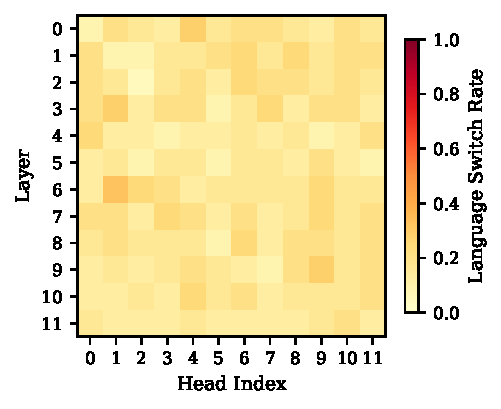
\includegraphics[width=\linewidth]{figures/fig1_ablation_heatmap.pdf}
    \end{minipage}\hfill
    \begin{minipage}[t]{0.49\textwidth}
        \centering
        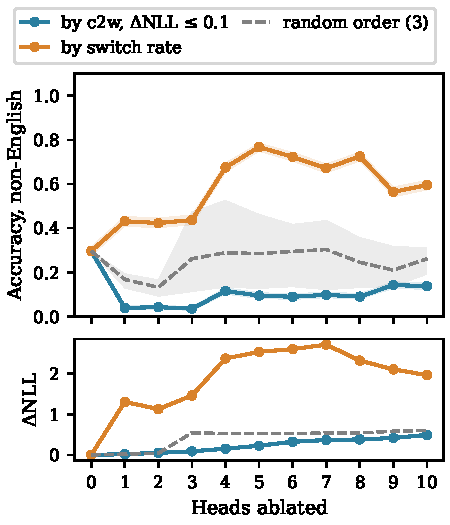
\includegraphics[width=\linewidth]{figures/fig3_accuracy_curve.pdf}
    \end{minipage}
    \caption{\textbf{GPT-2 head-level language identity and distributed
    robustness.} \textbf{(a)} Language switch rate across all 144 GPT-2
    attention heads. A small cluster spanning layers 0--10 shows
    disproportionate causal influence. L6H1 leads at 0.32 (99.3rd
    percentile, 3.23$\sigma$ above mean); a second tier (L0H4, L3H1,
    L9H9) sits at 0.28. \textbf{(b)} Language accuracy under progressive
    multi-head ablation (2,500-prompt evaluation, 95\% bootstrap CIs).
    Monotonic gradual degradation---without reaching chance in the tested
    sequence---is consistent with redundant or distributed encoding. Dotted line:
    chance (0.20).}
    \label{fig:gpt2_ablation}
\end{figure*}

\label{sec:multi}
Figure~\ref{fig:gpt2_ablation}(b) shows
accuracy under progressive multi-head ablation on the full 2,500-prompt
European set. Baseline accuracy is 43.5\%~[0.416, 0.454]. Ablating L6H1
alone reduces accuracy to 39.2\%~[0.373, 0.411]; ablating the top ten
heads reduces it to 32.4\%~[0.306, 0.343], an 11.1-point total
reduction. Critically, accuracy \textbf{never falls below chance
(20\%)} and degradation is monotonic, which is consistent with redundant or distributed
encoding; the result does not by itself establish a specific circuit
structure.

\paragraph{Attention redistribution following ablation.} The top-5 mean first-token attention delta
exceeds the permutation null for all three ablated heads
($p<10^{-5}$); the largest increases cluster \emph{above} the ablated layer
(layer-clustering $p<0.006$; full table in
Appendix~\ref{app:compensation}). Ablating L0H4 (layer~0) recruits
layer~2; ablating L6H1 (layer~6) recruits layers~7--9; ablating L9H9
(layer~9) recruits layers~10--11. The pattern is compatible with downstream
compensation, but it does not by itself establish a feedforward causal cascade. Amplifying individual top heads by $2\times$--$5\times$ produces no
observed accuracy improvement at the tested scales. Thus, simple amplification
of an individual head was insufficient to recover language accuracy in this
experiment; this result is motivated by prior inference-time representation
interventions, but does not directly test the intervention proposed in
\citet{li2023}.

\section{Results: First-Token Broadcasting and Probing}
\label{sec:attention}

Figure~\ref{fig:attn_comparison} (Appendix~\ref{app:attention_patterns}) shows
L6H1's attention on correct and confused prompts: every query position
attends to the first token at weight 0.62--1.00. Broadcaster heads
attend to the first prompt token with mean weight 0.85--0.89 across
generation steps, with stable low entropy across all 40 steps (mean 1.11
vs.\ 1.34 for random heads; Appendix~\ref{app:entropy}). Confused
prompts show \emph{higher} first-token attention in L6H1 (0.923 vs.\
0.847 on correct prompts): confusion does not simply coincide with loss of first-token access,
suggesting that downstream processing may determine the effective use of this
information. A descriptive taxonomy of heads (broadcaster vs.\ distributed) is given in
Appendix~\ref{app:taxonomy}.

\label{sec:probing}
In GPT-2, probing accuracy rises from 36\% at the embedding layer to
96\% at layers~10--11; in BLOOM, it reaches 100\% at layers~18--24.
Layers containing top causal heads show substantially higher probing
accuracy in both models (GPT-2: 85\% vs.\ 58\%; BLOOM: top-switch
layers all above 92\%), providing convergent evidence that language information is decodable in
layers containing larger causal effects, although probing alone does not
establish that the probed feature is causally responsible.

\section{Results: Training Regime and Language-Family Specificity}
\label{sec:qwen}

We apply LIHA to Qwen2.5-1.5B-Base and Qwen2.5-1.5B-Instruct---matched
in architecture and parameter count, with the same GQA configuration but
having different training histories---sweeping all 336 heads with 125 prompts. The \textbf{base model} is nearly flat: mean SR$=$0.0036
($\sigma{=}0.0046$), maximum SR$=$0.016 (L0H0), and 200/336 heads at
SR$=$0.0, indicating that, under single-head ablation and this sample size, causal
effects on detected output language are not strongly localized to any
individual head. The \textbf{instruct model} is qualitatively
different: L0H5 leads at SR$=$0.224 [0.152, 0.296], 8.93$\sigma$ above
the population mean---a 14$\times$ increase in max SR over the base
model. All 12 layer-0 heads are elevated (layer-0 mean SR$=$0.093 vs.\
0.023 for layers~1--27); six heads exceed SR$=$0.1
(Table~\ref{tab:qwen_top}). No language-switch events were observed for English under the tested
ablations in either variant; German
is most vulnerable (switch rate up to 0.44), replicating the
language-specificity pattern observed in GPT-2.

\paragraph{Cross-model comparison.} Table~\ref{tab:crossmodel}
summarizes all models. The progression from GPT-2 (distributed, middle layers) to Qwen-Base
(near-uniform) to Qwen-Instruct (layer-0 concentrated) is consistent with a
reorganization associated with the post-training regime. Because the Qwen
comparison contains only one base/instruct pair and the variants differ in
training history beyond a single isolated intervention, it does not by itself
establish instruction tuning as the causal ingredient.

\begin{table*}[t]
\caption{\textbf{Cross-model comparison of language identity
organization.}}
\label{tab:crossmodel}
\centering\small
\begin{tabular}{lcccc}
\toprule
\textbf{Property} & \textbf{GPT-2} & \textbf{BLOOM-1b7} & \textbf{Qwen-1.5B Base} & \textbf{Qwen-1.5B Instruct} \\
\midrule
Heads swept       & 144   & 128$^{\dagger}$ & 336   & 336   \\
Max SR            & 0.32  & 0.16            & 0.016 & 0.224 \\
Top head $\sigma$ & 3.23  & 2.60            & 2.70  & 8.93  \\
\# heads SR$>$0.1 & 15    & 4               & 0     & 6     \\
Critical layers   & 0--10 & 0--21           & none  & 0     \\
English switch events & none & none & none & none \\
\bottomrule
\end{tabular}
\smallskip

{\footnotesize $^{\dagger}$Every 3rd layer sampled; 128 of 384 heads.}
\end{table*}

\label{sec:extended}
Extending to Chinese (zh) and Russian (ru), the top European heads
(L6H1, L0H4, L3H1, L9H9; switch rates 0.28--0.32) produce SR$=$0.0 on
both---the European-language broadcaster heads show no observed switch effects on
the tested Chinese and Russian prompts. Different heads, concentrated in layers~0--4, govern
non-European languages instead---the same broad early-layer locus as
the instruction-tuned Qwen model (full breakdown in
Appendix~\ref{app:language_family}). Notably, L1H10, a \emph{distributed}
head, retains a non-trivial switch rate on both Chinese and Russian
(0.20) where the European broadcasters show no observed switch effects,
suggesting that some distributed heads may have broader cross-lingual effects
than the localized heads in this experiment.

\section{Discussion}
\label{sec:discussion}

\paragraph{A training-regime hypothesis.} Pretrained-only GPT-2 distributes
the language signal across 10+ middle-layer heads, while BLOOM shows similarly
broad effects in the sampled layers. Qwen-Instruct instead shows stronger
layer-0 concentration than the matched Qwen-Base model. This pattern is
consistent with an association between the post-training regime and circuit
localization, but the single base/instruct pair does not isolate instruction
tuning as the causal ingredient.

\paragraph{The early-layer convergence.} Chinese and Russian in GPT-2
recruit heads concentrated in layers~0--4; Qwen-Instruct concentrates
tightly at layer~0 specifically; and the Qwen base model's single
strongest head is also at layer~0. These early layers sit closest to
the tokenizer, where tokenization and prompt formatting can expose
language-correlated information early. Models that resolve language identity
early may therefore show effects in this broad locus, although the present
experiments do not establish a common causal origin, and the GPT-2
non-Latin-script effect is diffused across a four-layer window rather
than sharply localized to a single head the way the Qwen-Instruct
effect is.

\paragraph{Implications for inference-time intervention.} Ablating
ten heads causes only 11.1 points of monotonic, never-at-chance
accuracy decline, hierarchically absorbed downstream. Qwen-Instruct's layer-0 concentration raises the possibility that some
instruction-tuned models may be more amenable to targeted intervention, but
our results do not establish greater intervention reliability. More broadly,
the observed variation across GPT-2, Qwen-Base, and Qwen-Instruct indicates
that a single-head intervention may not transfer across training regimes or
language sets.

\paragraph{Future directions.} Path patching \citep{wang2022interpretability}
would distinguish heads that promote the target language from those
that suppress alternatives. Whether the layer-0 concentration in
Qwen-Instruct extends to larger instruction-tuned models, and whether
it enables more reliable language control, are open questions.

\paragraph{Overall interpretation.} Our results support a narrower conclusion
than a single universal language-identity circuit. In GPT-2, several heads
have measurable causal influence on output language, and a subset combine this
influence with persistent attention to the first prompt token. Localization and
effect magnitude vary across models, training regimes, and language sets.
These observations are consistent with language-related computation being
implemented by partially distributed, model-dependent circuits rather than a
single universal head-level mechanism.

\section{Limitations}
\label{sec:limitations}

GPT-2 switch rates use 500 prompts per European language; Qwen uses
125, useful for the base-vs.-instruct comparison but with a minimum
resolvable nonzero switch rate of $1/125\approx0.008$, so the large
number of Qwen-Base heads at SR$=$0.0 (200/336) partly reflects
measurement resolution. Zero-ablation cannot distinguish heads
promoting the correct language from those suppressing alternatives; we
compared this intervention with mean ablation as a sensitivity analysis, which
showed only a weak (though statistically significant) negative rank
correlation with zero-ablation rankings (Spearman
$\rho{=}{-}0.24$, $p{<}0.01$)---full analysis in
Appendix~\ref{app:limitations}.
Qwen2.5-1.5B's Grouped Query Attention means zeroing a Q-head slice has
different internal semantics than in standard MHA, since multiple Q-heads share
KV projections. Our intervention zeros the selected post-projection Q-head
output slice; the implications of this intervention for GQA-specific circuit
semantics require further validation. The Qwen comparison controls for
architecture and scale but spans a single model family; broader
replication across instruction-tuned families is needed to generalize
the training-regime hypothesis. Finally, our Chinese/Russian comparison
confounds \emph{script} (non-Latin orthography) with broader
\emph{typological} distance (morphology, word order, syntactic
structure): both languages differ from the European set on both
dimensions simultaneously, so we cannot yet attribute the early-layer
shift to script identity specifically versus typological distance more
generally. Disentangling these would require testing a Latin-script
language that is typologically distant from the European set (e.g.,
Vietnamese) alongside a non-Latin-script language that is typologically
close to it (e.g., Serbian in Cyrillic), which we leave to future work.

\paragraph{Responsible use.} This work analyzes publicly available pretrained
models with constructed prompts; no personal data is involved. \textbf{Positive
impact:} understanding first-token broadcasting could inform more reliable
multilingual systems and targeted mitigations for language-switching failures.
\textbf{Potential negative impact:} causal head-localization methods could
also be used to alter a model's language behavior in unintended ways, and the
layer-0 concentration observed in the instruction-tuned model may make some
interventions easier to target. \textbf{Mitigation:} we report aggregate
statistics rather than a ready-to-use intervention procedure, and the same
localization that may improve understanding of a mechanism can also support
monitoring and hardening. \textbf{Acknowledgement:}
Omitted for anonymous review.

\bibliography{references}

\clearpage

\appendix

\section{GPT-2 Ablation, Redundancy, and Compensation}
\label{app:gpt2}

\subsection{Full GPT-2 Ablation Sweep}
\label{app:full_sweep}

\begin{table}[H]
\caption{All GPT-2 heads with switch rate $> 0.15$.}
\label{tab:full_sweep}
\centering\small
\begin{tabular}{lcc}
\toprule
\textbf{Head} & \textbf{Switch Rate} & \textbf{Delta Acc.} \\
\midrule
L6H1   & 0.32 & $+$0.04 \\
L0H4   & 0.28 & $+$0.04 \\
L9H9   & 0.28 & $-$0.12 \\
L3H1   & 0.28 & $+$0.00 \\
L10H4  & 0.24 & $-$0.08 \\
L9H11  & 0.24 & $-$0.04 \\
L8H6   & 0.24 & $+$0.00 \\
L9H4   & 0.24 & $+$0.00 \\
L7H3   & 0.24 & $-$0.04 \\
L1H0   & 0.24 & $+$0.08 \\
L1H10  & 0.24 & $+$0.04 \\
L5H1   & 0.24 & $+$0.00 \\
L6H8   & 0.24 & $-$0.04 \\
L3H4   & 0.20 & $-$0.04 \\
L4H11  & 0.20 & $+$0.00 \\
\bottomrule
\end{tabular}
\end{table}

\subsection{Attention Redistribution Following Ablation}
\label{app:compensation}

\begin{table}[H]
\caption{\textbf{Heads with the largest increases in first-token attention
when L6H1 is ablated.} These heads show positive attention deltas; the set
clusters in layers 7--9, above the ablated layer~6 ($p{=}0.002$). Because many
heads are tested and the displayed heads are selected by effect size, we do
not interpret the uncorrected per-head $p$-values as confirmatory evidence.}
\label{tab:compensatory}
\centering\small
\begin{tabular}{lrrrr}
\toprule
\textbf{Head} & \textbf{Base} & \textbf{Ablated} & $\boldsymbol{\Delta}$ & $\boldsymbol{z}$ \\
\midrule
L9H8  & 0.267 & 0.275 & $+$0.007 & $3.45^{**}$ \\
L7H3  & 0.745 & 0.751 & $+$0.006 & $3.01^{**}$ \\
L7H10 & 0.873 & 0.879 & $+$0.006 & $2.70^{**}$ \\
L7H1  & 0.833 & 0.838 & $+$0.005 & $2.65^{**}$ \\
L7H6  & 0.702 & 0.705 & $+$0.003 & $2.10^{*}$  \\
\bottomrule
\end{tabular}
\smallskip

{\footnotesize $^{**}p{<}0.01$;\enspace$^{*}p{<}0.05$;\enspace permutation test, $n{=}100{,}000$.}
\end{table}

\subsection{Per-Language Switch Rates}
\label{app:perlang}

\begin{table}[H]
\caption{Per-language switch rates for the top five GPT-2 heads from
Table~\ref{tab:top_heads}, computed on the 5 hand-written
sentence-starter prompts per language (\S\ref{sec:setup}).}
\label{tab:per_language_app}
\centering\small
\begin{tabular}{lccccc}
\toprule
\textbf{Head} & \textbf{EN} & \textbf{FR} & \textbf{DE} & \textbf{ES} & \textbf{IT} \\
\midrule
L6H1  & 0.0 & 0.2 & 0.2 & 0.4 & 0.6 \\
L0H4  & 0.0 & 0.2 & 0.2 & 0.4 & 0.4 \\
L3H1  & 0.0 & 0.2 & 0.2 & 0.4 & 0.4 \\
L9H9  & 0.0 & 0.2 & 0.0 & 0.4 & 0.6 \\
L7H3  & 0.0 & 0.2 & 0.2 & 0.2 & 0.4 \\
\bottomrule
\end{tabular}
\smallskip

{\footnotesize Note: this qualitative breakdown uses the 5 hand-written
prompts per language and therefore differs slightly from the aggregate
switch rates over the full 500-prompt set reported in
Table~\ref{tab:top_heads}.}
\end{table}

\section{First-Token Broadcasting Diagnostics}
\label{app:broadcasting}

\subsection{Attention Patterns on Correct and Confused Prompts}
\label{app:attention_patterns}

\begin{figure}[H]
    \centering
    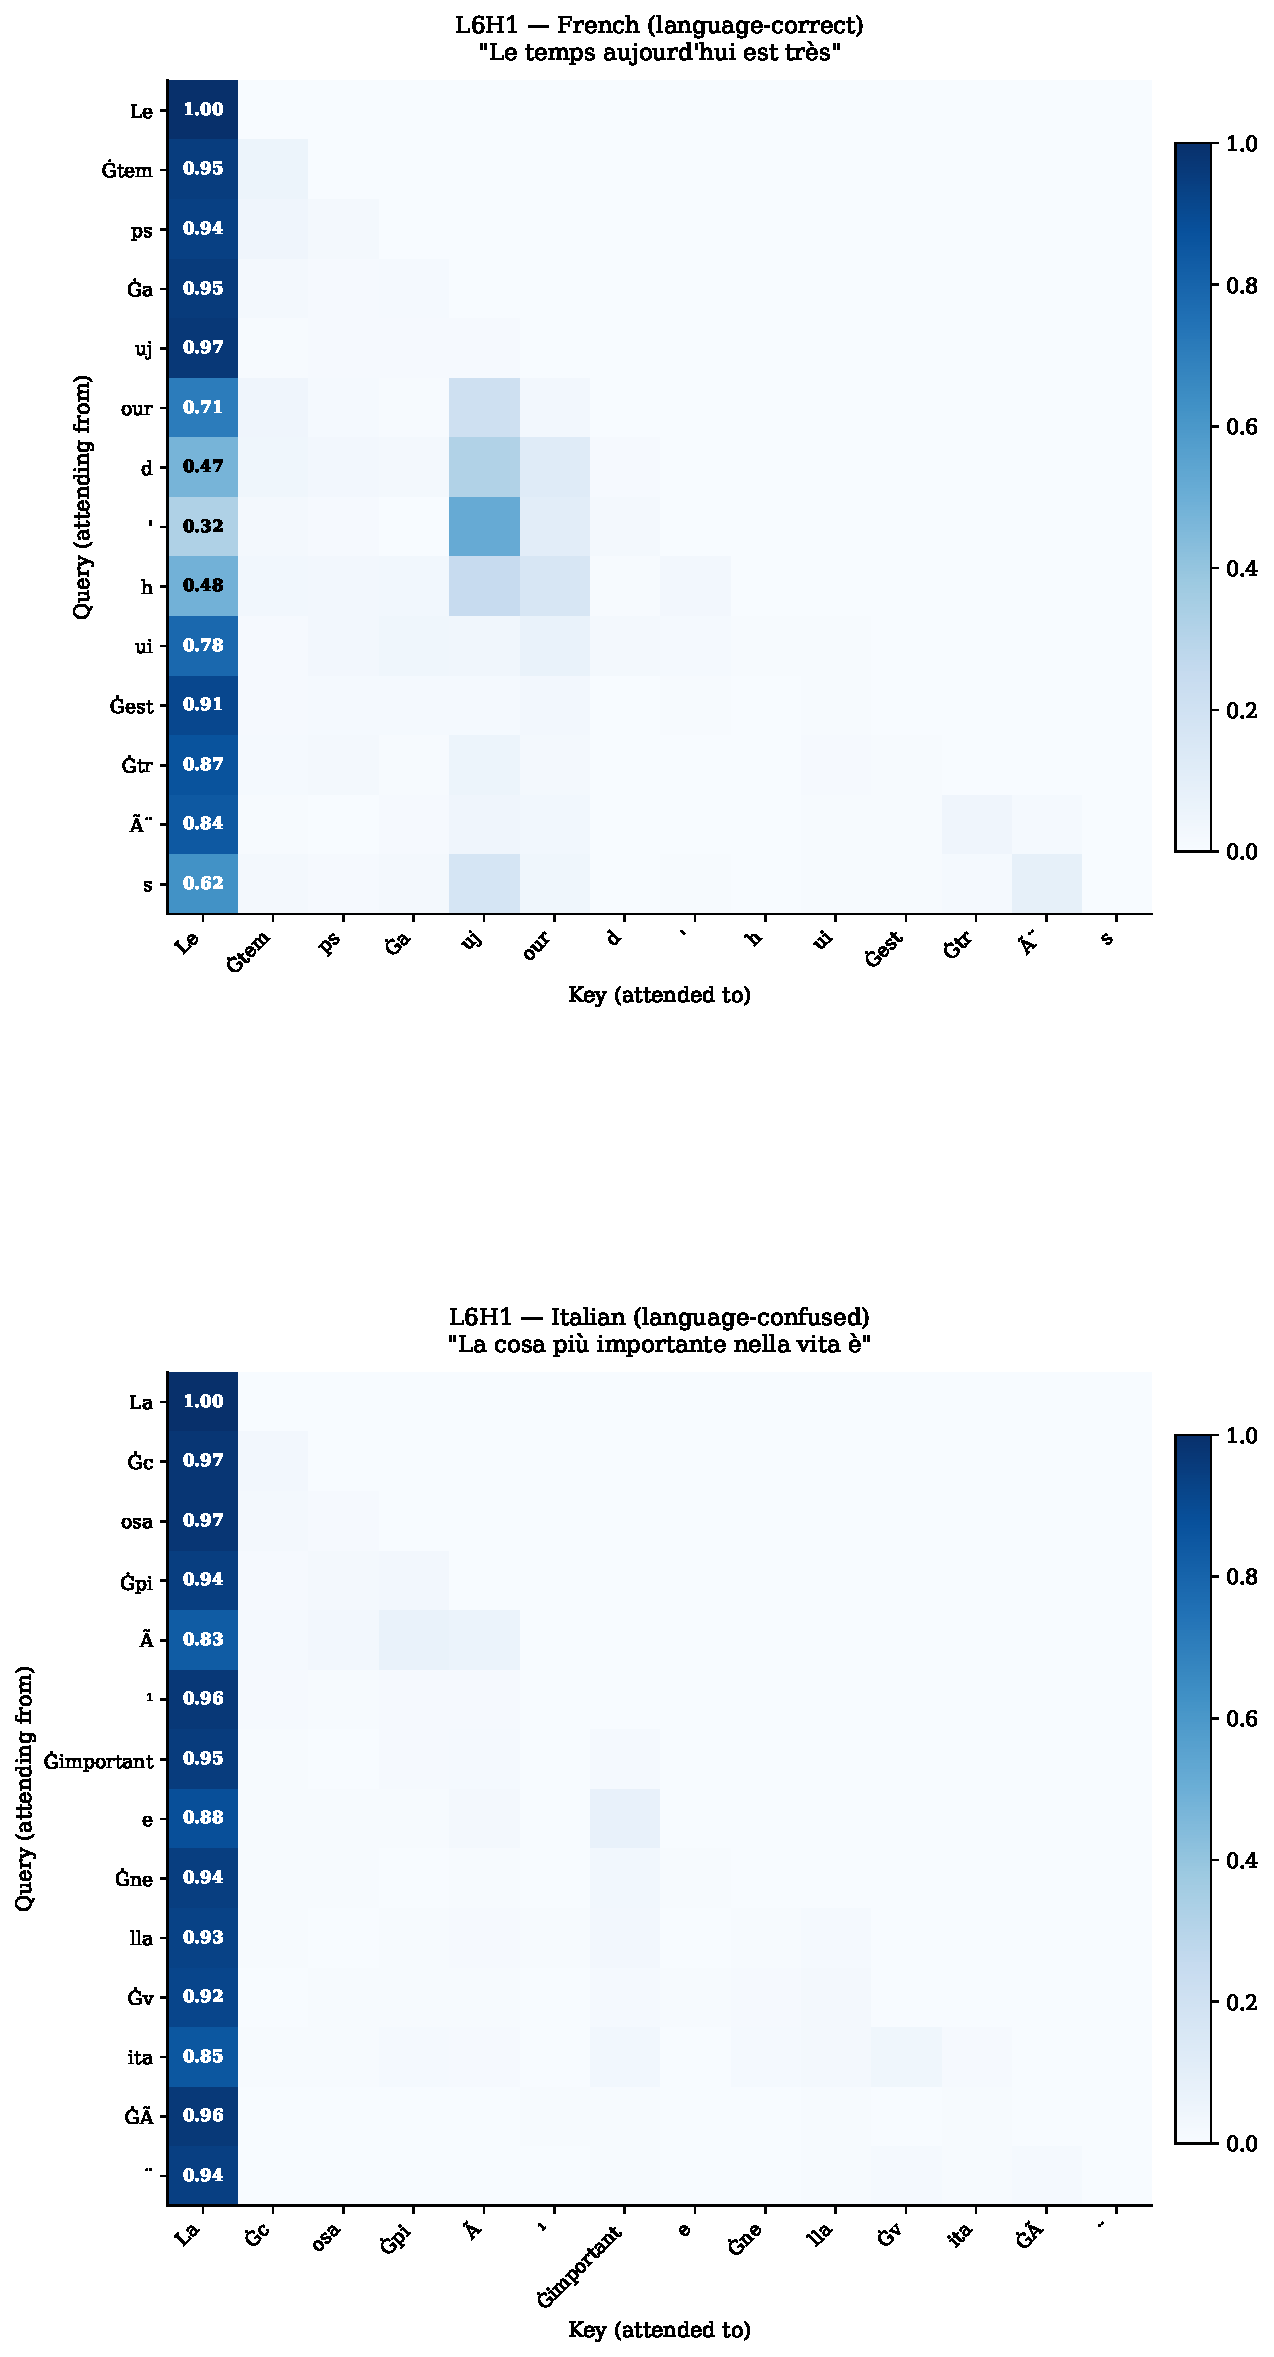
\includegraphics[width=0.55\columnwidth]{figures/fig_attention_comparison.pdf}
    \caption{\textbf{L6H1 attention on a correct French prompt (left)
    and confused Italian prompt (right).} First-token focus is consistent
    in both cases; confusion arises downstream.}
    \label{fig:attn_comparison}
\end{figure}

\subsection{Entropy Over Generation Time}
\label{app:entropy}

\begin{figure}[H]
    \centering
    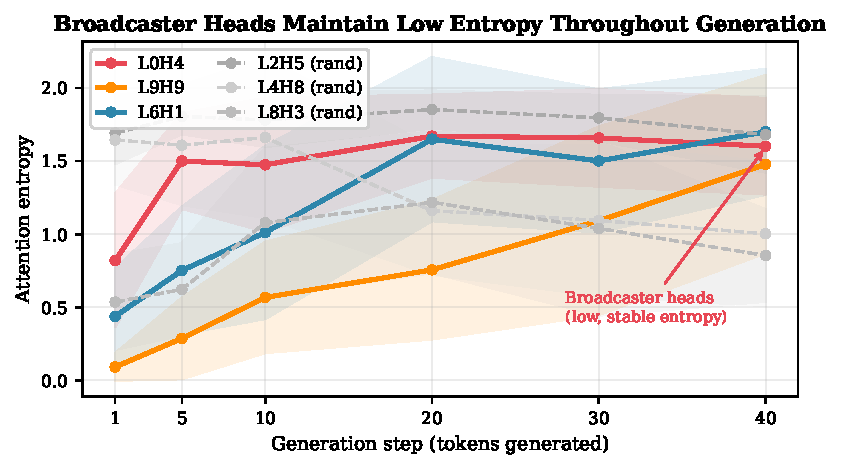
\includegraphics[width=\columnwidth]{figures/fig_entropy_over_time.pdf}
    \caption{\textbf{Attention entropy over generation steps.}
    Broadcaster heads (solid) maintain lower entropy (mean 1.11) than
    random heads (dashed, mean 1.34) across all 40 steps.}
    \label{fig:entropy}
\end{figure}

\subsection{Functional Taxonomy of Language-Critical Heads}
\label{app:taxonomy}

\begin{table}[H]
\caption{\textbf{Descriptive taxonomy of top language-critical heads.}}
\label{tab:taxonomy}
\centering\small
\begin{tabular}{llcc}
\toprule
\textbf{Head} & \textbf{Type} & \textbf{First-Tok Attn} & \textbf{Entropy} \\
\midrule
L6H1  & Broadcaster & 0.876 & 0.517 \\
L10H4 & Broadcaster & 0.848 & 0.677 \\
L7H3  & Broadcaster & 0.892 & 0.538 \\
L1H10 & Distributed & 0.112 & 2.013 \\
\bottomrule
\end{tabular}
\end{table}

\section{Training-Regime and Language-Family Specificity}
\label{app:language_family}

\subsection{Top Qwen2.5-1.5B-Instruct Heads}
\label{app:qwen_top}

\begin{table}[H]
\caption{\textbf{Top five Qwen2.5-1.5B-Instruct heads} by switch rate
(125 prompts, 95\% bootstrap CIs). No language-switch events were observed for English under the tested single-head ablations.}
\label{tab:qwen_top}
\centering\small
\begin{tabular}{lccc}
\toprule
\textbf{Head} & \textbf{SR} & \textbf{95\% CI} & \textbf{$\sigma$ above mean} \\
\midrule
L0H5  & 0.224 & {[0.152, 0.296]} & 8.93 \\
L0H11 & 0.144 & {[0.088, 0.208]} & 5.33 \\
L1H9  & 0.136 & {[0.080, 0.200]} & 4.97 \\
L0H7  & 0.120 & {[0.064, 0.176]} & 4.25 \\
L1H7  & 0.112 & {[0.064, 0.168]} & 3.89 \\
\midrule
Population mean & 0.026 & -- & -- \\
\bottomrule
\end{tabular}
\end{table}

\subsection{European vs. Chinese/Russian Head Specificity}
\label{app:extended_table}

\begin{table}[H]
\caption{\textbf{European-language versus Chinese/Russian head effects.}
Left: top European-language heads show no observed switch events on the tested
Chinese/Russian prompts. Right: other heads show nonzero switch rates,
concentrated in layers 0--4. These small-sample results are descriptive and
do not isolate script from typology or tokenization.}
\label{tab:extended}
\centering\tiny
\begin{tabular}{lccc|lccc}
\toprule
\textbf{Head} & \textbf{EU} & \textbf{ZH} & \textbf{RU}
& \textbf{Head} & \textbf{All} & \textbf{ZH} & \textbf{RU} \\
\midrule
L6H1  & 0.32 & 0.00 & 0.00 & L0H0 & 0.40 & 0.20 & 0.60 \\
L0H4  & 0.28 & 0.00 & 0.00 & L4H5 & 0.30 & 0.40 & 0.20 \\
L3H1  & 0.28 & 0.00 & 0.00 & L4H2 & 0.30 & 0.40 & 0.20 \\
L9H9  & 0.28 & 0.00 & 0.00 & L0H1 & 0.20 & 0.00 & 0.40 \\
L1H10 & 0.24 & 0.20 & 0.20 & L0H7 & 0.20 & 0.20 & 0.20 \\
\bottomrule
\end{tabular}
\smallskip

{\footnotesize \textbf{All} denotes the mean switch rate averaged
across the Chinese and Russian prompt sets combined.}
\end{table}

\subsection{Extended Language Prompts}
\label{app:prompts}

\begin{table}[H]
\caption{Chinese and Russian prompts used in the extended language
experiments. Russian is shown in transliteration; Cyrillic originals
are in \texttt{data/prompts\_ru.csv}.}
\label{tab:extended_prompts}
\centering\small
\begin{tabular}{lp{5.5cm}}
\toprule
\textbf{Lang} & \textbf{Prompt} \\
\midrule
zh & \begin{CJK}{UTF8}{gbsn}今天的天气非常\end{CJK} \\
zh & \begin{CJK}{UTF8}{gbsn}我想告诉你关于\end{CJK} \\
zh & \begin{CJK}{UTF8}{gbsn}科学家们发现了\end{CJK} \\
zh & \begin{CJK}{UTF8}{gbsn}生活中最重要的事是\end{CJK} \\
zh & \begin{CJK}{UTF8}{gbsn}从前有一个\end{CJK} \\
\midrule
ru & \textit{Segodnya pogoda ochen\textquotesingle} \\
ru & \textit{Ya khotel by rasskazat\textquotesingle{} vam o} \\
ru & \textit{Uchyonye obnaruzhili, chto} \\
ru & \textit{Samoye vazhnoye v zhizni~--- eto} \\
ru & \textit{Odnazhdy zhil-byl} \\
\bottomrule
\end{tabular}
\end{table}

\section{Statistical Test Details}
\label{app:bootstrap}

Switch rate CIs use 10,000 bootstrap samples (resampling with
replacement, 2.5th/97.5th percentiles). Attention redistribution following ablation
uses 100,000-sample permutation tests: the observed top-5 mean delta
is compared against the distribution of top-5 means from 100,000
random draws of size 5 from the full 143-head delta population.
Layer-clustering tests compare observed layer entropy of the five largest
attention-increase heads against the entropy from 100,000 random 5-head draws.

\section{Mean-Ablation Methodological Check}
\label{app:limitations}

We additionally attempted mean ablation---replacing each head's output
with its mean activation across the dataset---as a methodological
check. The resulting switch rates showed only a weak negative rank correlation with
zero-ablation rankings (Spearman $\rho{=}{-}0.24$, $n{=}144$ heads),
statistically distinguishable from zero at $p{<}0.01$ under the standard
large-sample approximation for Spearman's $\rho$. We treat this as a
sensitivity analysis rather than evidence that either intervention is
universally preferable. The sign and magnitude are consistent with the two
interventions perturbing different aspects of the representation, but the
present analysis does not establish why the rankings differ. In particular,
we do not use this result to confirm that zero-ablation is uniquely
appropriate; zero-ablation is retained as the primary intervention because it
provides a direct removal of the head's post-projection residual contribution.

\end{document}
